\section{Results}\label{sec:results}

\subsection{When conversion raises the total as capital land declines}\label{sec:mask}

At a fixed quality state $q$, the annual value of capital land per hectare, $\Ups(q)$, has a concave quadratic shape. It is highest at $q^*=q_{\max}/2$; under the baseline parameters this maximum is $0.066$\,gha\,ha$^{-1}$. Of that amount, $0.016$ comes from quality growth and $0.05$ from direct yield, so regeneration adds a modest contribution in this case.

The immediate effect of conversion depends on the difference between the annual account contribution of a hectare of fast land and the effective value of a hectare of capital land. We call this the \emph{composition diagnostic}:
\begin{equation}\label{eq:dconv}
\dconv(q,D)=b_f(D)-\Ups(q).
\end{equation}
At baseline parameter values, $\dconv$ is $+0.787$, $+0.784$, and $+0.794$\,gha\,ha$^{-1}$ at $q=0.3$, $0.6$, and $0.9$, respectively. All three values lie in the composition-premium regime ($\dconv>0$), where conversion contributes positively to the aggregate at the margin. At $\dconv=0$, the contribution is first-order neutral (composition-neutrality); at $\dconv<0$, it is negative (composition-discount). These names classify the conversion term alone: maintenance, retirement, quality change, and other terms still affect the net change in $B$. At fixed $q$, capital-land contribution is linear in $A_c$, so it has no interior maximum as capital-land area changes.

\begin{proposition}[Conversion, aggregate change, and what the total can reveal]\label{prop:mask}
Let $T_b\equiv0$, $R_{rc}\equiv0$ and hold $D$ fixed, so that $b_f$ is constant. Along any solution of \eqref{eq:B}--\eqref{eq:q},
\begin{equation}\label{eq:identity}
\dot B=\dconv(q)\,u_c+b_f\big(\mu A_r-\eta_f A_f\big)+b_{G,c}\,G_c'(q)\,A_c\,\dot q .
\end{equation}
\begin{enumerate}[label=(\roman*)]
\item During conversion ($u_c>0$), capital-land area falls when restoration is off. The conversion term in the rate of change of $B$ is $\dconv(q)u_c$; it is positive exactly when $\dconv(q)>0$. It determines the sign of the net change only when maintenance and retirement balance ($\mu A_r=\eta_fA_f$) and quality is not changing ($\dot q=0$).
\item In the reduced comparison with fixed demand and fixed debt, baseline availability shares, balanced maintenance and retirement, and no quality change, a positive $\dconv$ makes the shortfall fall as conversion proceeds. The shortfall reaches zero if the balance is reached first. If the minimum-area constraint binds first, $A_c$ approaches $\Acmin$ and a shortfall can remain. This result does not apply unchanged when the other terms in the full model are active.
\item At fixed $b_f>0$ and $q$, the total $B=b_fA_f+\Ups(q)A_c$ gives one equation for the two land areas $A_f$ and $A_c$. Near an interior state, a small change in $A_c$ can be offset by $\delta A_f=-(\Ups/b_f)\delta A_c$ and $\delta A_r=-\delta A_f-\delta A_c$, preserving both $B$ and total area as long as land bounds are respected. Thus nearby land allocations can produce the same total, and $B$ alone does not identify $A_c$. For a finite observed change $\Delta B$, the offset is $\Delta A_f=(\Delta B-\Ups\Delta A_c)/b_f$; it is feasible only when all resulting areas remain within their bounds, so the range depends on the starting state. If $A_f$ and $b_f$ are observed independently, the residual $C=B-b_fA_f=\Ups(q)A_c$ identifies their product, not the area and value separately. An independent observation of $A_c$ would give $\Ups(q)=C/A_c$. A single value of $\Ups$ cannot separate $b_c$, $b_{G,c}$, $\rho_c$, and $q$; even with informative independent observations of $q$, it identifies at most $b_c$ and the product $b_{G,c}\rho_c$, not $b_{G,c}$ and $\rho_c$ separately.
\end{enumerate}
\end{proposition}

\begin{proof}
Differentiate \eqref{eq:B} with $b_f$ constant and substitute \eqref{eq:Ac}--\eqref{eq:Af} with $R_{rc}=0$: $\dot B=b_f(u_c+\mu A_r-\eta_fA_f)-\Ups u_c+b_{G,c}G_c'(q)A_c\dot q$, which is \eqref{eq:identity}. (i) Follows from \eqref{eq:identity} with $R_{rc}=0$; when the maintenance--retirement imbalance and quality-growth terms vanish, only the conversion term remains. (ii) Under the reduced-case conditions in the statement, $S=E-B$ and $\dot S=-\dot B=-\dconv u_c<0$ on $S>0$. Since $S$ is bounded below by zero and $A_c$ is bounded below by $\Acmin$, conversion either closes the shortfall or is limited by the floor. (iii) At fixed $b_f$ and $q$, the observation map is linear; an interior feasible point admits the stated small perturbations along a level set of $B$, while finite changes must also obey the area bounds. The residual $C$ identifies only $\Ups(q)A_c$ unless $A_c$ is independently observed; the parameter combination follows from the definition of $\Ups(q)$.
\end{proof}

Figure~\ref{fig:model}a shows the baseline run with frozen demand $E=0.825$\,gha and restoration switched off. It starts with $A_f=0.6$\,ha, $A_c=1.5$\,ha, $A_r=0.4$\,ha, and $q=0.9$. During conversion, total model biocapacity $B$ rises from $0.594$ to $0.825$\,gha ($39\%$), capital-land area falls from $1.500$ to $0.808$\,ha ($46\%$), and fast-land area rises from $0.600$ to $0.923$\,ha.

The quality state $q$ rises from $0.9$ to $1.0$. Because it starts above $q^*=0.5$, the peak of $\Ups(q)$, its per-hectare value falls from $0.05576$ to $0.05000$\,gha\,ha$^{-1}$. The modeled contribution $\Ups(q)A_c$ therefore falls from $0.08364$ to $0.04038$\,gha ($51.7\%$). This decline is larger than the $46.2\%$ decline in area because per-hectare value also falls. The land transfers conserve area: $\Delta A_f+\Delta A_c+\Delta A_r=0$.

The change is fastest at first, then slows. In the deficit-side model, the approach to balance is exponential, with a slow rate $|\lambda_1|=0.054$\,yr$^{-1}$—an e-folding time of about $19$\,yr. Within $25$\,yr, $98\%$ of the rise in $B$ and $85\%$ of the decline in $A_c$ have occurred ($B=0.820$\,gha and $A_c=0.913$\,ha); $97\%$ of the area decline has occurred by year $50$. The simultaneous pattern $\dot B>0$ and $\dot A_c<0$ lasts about $149$\,yr at the numerical resolution used.

The long tail reflects reserve adjustment. As fast land retires to the reserve, its contribution falls and a small shortfall reopens, allowing more conversion until $A_r/A_f=\eta_f/\mu$. The duration is therefore not a fixed horizon: its scale depends on the slow rate $\lambda_1$ and its size on $\dconv$ and the initial shortfall (SI~\S S2.2).

This result limits what an aggregate can tell us. Total $B$ alone cannot show whether capital land is shrinking while another component grows. Independent measures of fast-land area $A_f$ and yield $b_f$ let us calculate the remainder $C=B-b_fA_f$, but that remainder identifies only the capital-land contribution—not its area and per-hectare value separately. We call a trajectory with rising $B$ and falling $A_c$ a \emph{composition mask}. A distinct, though potentially overlapping, pattern is the \emph{liquidation mask}: demand $E$ remains steady while $A_c$ falls. The composition mask describes an aggregate-versus-area signature; the liquidation mask describes a demand-versus-area signature. The composition diagnostic $\dconv$ tells us the sign of conversion's marginal contribution, not necessarily the net change in $B$ when other terms are active. A liquidation mask does not require $\dconv>0$. Observing $B$, $E$, and $A_c$ distinguishes the two defining signatures. Here, “liquidation mask” names this trajectory; it is separate from the optional timber-liquidation extension, which is off in all reported runs.

\begin{figure}[!htbp]
\centering
\includegraphics[width=\textwidth]{fig1_model_dynamics}
\caption{Model results at the baseline parameter set (Table~\ref{tab:params}). Account amounts $B$ and $E$ are in gha; land areas are in ha; population is in cap. (a) Frozen demand $E=0.825$\,gha, restoration off, $A_{f0}=0.6$\,ha, $A_{c0}=1.5$\,ha, and $q_0=0.9$. $B$ rises from $0.594$ to $0.825$\,gha as $A_c$ falls from $1.500$ to $0.808$\,ha and $A_f$ rises from $0.600$ to $0.923$\,ha. Shading marks the interval with $\dot B>0$ and $\dot A_c<0$ (about $149$\,yr; only the first $60$\,yr are shown; within $25$\,yr, $98\%$ of the rise in $B$ and $85\%$ of the fall in $A_c$ occur). (b) Fixed-demand balance relation $B_{eq}(A_c)$ and its calculated areas $A_c^*(E)=1.110$, $0.626$, $0.385$, $0.143$, and $0.070$\,ha at $E=0.70$, $0.90$, $1.00$, $1.10$, and $1.13$\,gha. The curve meets the minimum $A_c=0.05$\,ha at $\Eceil\approx1.138$\,gha; above this demand, no balance point is admissible. (c) Endogenous-demand runs with $\tau_g=20$\,yr, $\tau_p=25$\,yr, and $\chi_r=0.10$\,gha$^{-1}$\,yr$^{-1}$. For each starting area $A_{c0}$, the minimum area reached varies continuously and monotonically with initial population $P_0$ (initial demand $E_0=eP_0$). The floor is approached asymptotically; triangles mark the proximity values in Table~\ref{tab:model}, defined by an approach to within $10^{-6}$\,ha. No discontinuity is observed.}
\label{fig:model}
\end{figure}

\subsection{Fixed demand leads to a minimum-area boundary, not a fold}\label{sec:ceiling}

When population has adjusted to the model's carrying capacity, $P=K=B/e$, so demand $E=eP$ equals biocapacity $B$ and the shortfall is zero. Active conversion is therefore transient in the endogenous-population runs. To study how the balance changes with demand, we also hold $E$ fixed and analyze the reduced land system. The model imposes a minimum capital-land area $\Acmin$; this is a \emph{typed floor}, a limit on one specific land class rather than on the aggregate.

\begin{proposition}[Balance point, demand ceiling and affine deficit-side dynamics]\label{prop:ceiling}
For this reduced comparison, hold demand at $E$, switch off the technology boost and restoration, set debt $D=0$, and fix quality at $q=q_{\max}$. This quality is the attractor of \eqref{eq:q} for $q(0)>0$. Let $k=\mu/(\mu+\eta_f)$ and
\begin{equation}\label{eq:Beq}
B_{eq}(A_c)=b_{f0}\,k\,(A_{tot}-A_c)+b_cA_c=b_{f0}kA_{tot}-(b_{f0}k-b_c)A_c .
\end{equation}
\begin{enumerate}[label=(\roman*)]
\item With no conversion ($S=0$), reserve-to-fast maintenance balances fast-land retirement. This gives $A_f=k(A_{tot}-A_c)$ and $A_r=(1-k)(A_{tot}-A_c)$, where $k=\mu/(\mu+\eta_f)$. The resulting total is $B_{eq}(A_c)$. If $b_{f0}k>b_c$, this total decreases as $A_c$ increases, so there is at most one balance point $B_{eq}(A_c^*)=E$:
\begin{equation}\label{eq:Acstar}
A_c^*(E)=\frac{b_{f0}kA_{tot}-E}{b_{f0}k-b_c}.
\end{equation}
The algebraic solution is feasible when $B_{eq}(A_{tot})\le E\le\Eceil$, where $\Eceil=B_{eq}(\Acmin)$. It lies above the minimum area exactly when $E<\Eceil$. At lower demand, the algebraic root lies above $A_{tot}$, and every feasible no-conversion allocation already supplies at least $E$.
\item While shortfall is positive and conversion is not yet limited by the minimum-area constraint, the land subsystem is affine in $z=(A_f,A_c)$: $\dot z=Jz+c$, with
\begin{equation}\label{eq:J}
J=\begin{pmatrix}-\tconv^{-1}-\mu-\eta_f & -\mu-\dfrac{b_c}{b_f\tconv}\\[8pt] \tconv^{-1} & \dfrac{b_c}{b_f\tconv}\end{pmatrix},
\qquad \det J=\frac{\mu+\eta_f}{\tconv}\Big(k-\frac{b_c}{b_f}\Big),
\end{equation}
and $\operatorname{tr}J<0$. The matrix does not depend on demand or on the current state. Its determinant is positive exactly when $B_{eq}$ decreases, and its fixed point is the balance point in (i). For $B_{eq}(A_{tot})\le E<\Eceil$, trajectories that remain in this regime approach that point at rates set by the eigenvalues of $J$. For $E>\Eceil$, the balance point would lie below the allowed minimum: $A_c$ approaches $\Acmin$ asymptotically and the shortfall tends to $S^*=E-\Eceil>0$. Thus the reduced balance curve meets the minimum-area boundary; it does not turn back or form a fold. The leading eigenvalue does not approach zero at $E=\Eceil$, and the reduced equilibrium relation has no hysteresis. These conclusions hold under the stated assumptions and do not imply that the realized land allocation is independent of its history.
\item Above the demand ceiling, with degradation active, debt approaches a unique value $D^*(E)$ satisfying $\eta D=E-B_{eq}(\Acmin;D)$, where $B_{eq}(\cdot;D)$ uses yield $b_{f0}e^{-\alpha D}$. This result requires $\eta>\alpha b_{f0}k(A_{tot}-\Acmin)$; the equilibrium debt increases with demand.
\end{enumerate}
\end{proposition}

\begin{proof}
(i) With $S=0$ and $R_{rc}=0$, \eqref{eq:Af} gives $\mu A_r=\eta_fA_f$, hence $A_r/A_f=\eta_f/\mu$ and, with $A_r=A_{tot}-A_f-A_c$, $A_f=k(A_{tot}-A_c)$; substituting into \eqref{eq:B} with $q=q_{\max}$ ($\Ups=b_c$) and $D=0$ gives $B=B_{eq}(A_c)$, and $S=0$ requires $B\ge E$. Strict monotonicity and \eqref{eq:Acstar} follow from $b_{f0}k>b_c$. (ii) On the deficit side $u_c=(E-b_fA_f-b_cA_c)/(b_f\tconv)$ is affine in $z$; substituting into \eqref{eq:Ac}--\eqref{eq:Af} with $A_r=A_{tot}-A_f-A_c$ gives $J$ and a constant vector $c$ by direct differentiation; $\det J$ follows by expansion, and $\operatorname{tr}J=-\tconv^{-1}(1-b_c/b_f)-\mu-\eta_f<0$ for $b_c<b_f$. The fixed point solves $u_c=0$ and $\mu A_r=\eta_fA_f$, i.e.\ it is the balance point. Because $J$ is constant, convergence rates are constant along the branch. (iii) The map $D\mapsto\eta D+B_{eq}(\Acmin;D)-E$ is continuous, negative at $D=0$ when $E>\Eceil$, tends to $+\infty$, and is strictly increasing when $\eta>\alpha b_{f0}k(A_{tot}-\Acmin)\ge-\partial_DB_{eq}$; hence it has a unique root, which increases with $E$.
\end{proof}

The uniqueness result is about the reduced equilibrium relation, not path independence of realized states. In the baseline trajectory, $R_{rc}=0$ and the conversion flow $u_c$ has no reverse counterpart. When the shortfall closes, $A_c$ stops declining and approaches its lower balance value; it remains below its pre-overshoot level because this run contains no restoration flow. The quality state $q$ evolves separately and can continue changing $\Ups(q)$ even as $A_c$ settles. Thus the model has a unique frozen-demand balance point under Proposition~\ref{prop:ceiling}'s restrictions, but a history-dependent post-overshoot land allocation; this is not perpetual decline at equilibrium and is not a general claim about real ecosystems.

At baseline, $k=0.5455$ and the slope $b_{f0}k-b_c=0.414$\,gha\,ha$^{-1}$. The demand ceiling is $\Eceil=1.138$\,gha. The predicted balance areas—$1.110$, $0.626$, $0.385$, $0.143$, and $0.070$\,ha at demands of $0.70$, $0.90$, $1.00$, $1.10$, and $1.13$\,gha—match the integrated equilibria (Fig.~\ref{fig:model}b). The eigenvalues of $J$ are real and negative: $\lambda_1=-0.0537$ and $\lambda_2=-0.998$\,yr$^{-1}$. Across the tested fast-land yields, $\lambda_1$ changes only from $-0.0522$ at $b_f=0.60$ to $-0.0556$\,yr$^{-1}$ at $b_f=2.00$ and never changes sign (Table~\ref{tab:model}a).

Above the ceiling, the calculated debt equilibria are $D^*=1.19$ and $5.38$\,gha\,yr at $E=1.158$ and $1.238$\,gha; numerical integrations give $1.21$ and $5.39$\,gha\,yr. The condition for a unique debt equilibrium holds with margin: $\alpha b_{f0}k(A_{tot}-\Acmin)=0.034$\,yr$^{-1}$, below $\eta=0.05$\,yr$^{-1}$. Thus debt saturates rather than growing without bound under fixed demand.

We use \emph{critical slowing down} in its standard sense: as a system approaches a fold, its slowest return rate tends to zero and the return time $T_{ret}\approx-1/\lambda_1$ grows. Here the linearization is constant along the reduced balance branch; $\lambda_1$ does not approach zero, and the return time stays near $19$\,yr as $E$ approaches $\Eceil$. The model's signal is instead $A_c$ approaching its minimum, which an aggregate-only observation cannot reveal.

With population responding to supply, the minimum capital-land area reached during a run varies continuously and monotonically with initial population $P_0$ for each starting area $A_{c0}$ (Fig.~\ref{fig:model}c). The floor is approached asymptotically, not crossed, because $u_c\le(A_c-\Acmin)/\tconv$. A larger starting area supports a larger initial population before the trajectory approaches the floor.

Table~\ref{tab:model}b reports the initial populations at which $A_c$ comes within $10^{-2}$, $10^{-4}$, or $10^{-6}$\,ha of its minimum. These are tolerance-based proximity values, not abrupt thresholds. At the tightest tolerance, the values are $P_0\approx2.41$, $2.70$, $2.98$, and $3.14$\,cap for starting areas $A_{c0}=0.40$, $0.70$, $1.00$, and $1.18$\,ha, respectively. They rise with starting area, and no jump appears at any of the tested tolerances.

For $A_{c0}=1.0$\,ha, the $10^{-6}$\,ha proximity value changes by at most $0.001$\,cap across regeneration delays $\tau_g=5$, $20$, and $40$\,yr (SI Table S2). This narrow comparison does not establish that delay has no effect outside the tested range. The threshold is also the same to three decimal places with surplus-gated restoration on or off (SI~\S S4), because that restoration is inactive while $B<E$.

\begin{table}[!htbp]
\centering\small
\caption{Model results at the baseline parameter set. (a) Composition diagnostic at $q^*=q_{\max}/2$ ($\Ups(q^*)=0.066$\,gha\,ha$^{-1}$), eigenvalues of the deficit-side matrix $J$ of \eqref{eq:J} and the demand ceiling, for a sweep of the fast-land yield $b_f$ (all other parameters at baseline). (b) Initial population $P_0$ (cap; $E_0=eP_0$ in gha, with $e=0.55$\,gha\,cap$^{-1}$) at which the minimum capital land reached during an endogenous-demand run ($A_{f0}=0.6$\,ha, dimensionless $q_0=0.9$, $\tau_g=20$\,yr, $\tau_p=25$\,yr) comes within the stated distance of the typed floor $\Acmin=0.05$; the first two columns are read from a $P_0$ grid of step $0.1$ ($\Delta t=0.1$\,yr, $T=400$\,yr), the last is a bisection using the $10^{-6}$\,ha floor-proximity criterion ($\Delta t=0.05$\,yr, $T=1000$\,yr). Drawdown depth is continuous in $P_0$ (Fig.~\ref{fig:model}c); the thresholds are a band, not a single value.}
\label{tab:model}
\begin{tabular}{l l l l l}
\toprule
\multicolumn{5}{l}{(a) Fast-land yield sweep (all rows composition-premium, $\dconv>0$)}\\
$b_f$ (gha\,ha$^{-1}$) & $\dconv(q^*)$ (gha\,ha$^{-1}$) & $\lambda_1$ (yr$^{-1}$) & $\lambda_2$ (yr$^{-1}$) & $\Eceil$ (gha) \\
\midrule
$0.60$ & $+0.534$ & $-0.0522$ & $-0.975$ & $0.804$ \\
$0.85$ (baseline) & $+0.784$ & $-0.0537$ & $-0.998$ & $1.138$ \\
$1.20$ & $+1.134$ & $-0.0547$ & $-1.014$ & $1.606$ \\
$2.00$ & $+1.934$ & $-0.0556$ & $-1.029$ & $2.675$ \\
\bottomrule
\end{tabular}

\medskip
\begin{tabular}{l l l l}
\toprule
\multicolumn{4}{l}{(b) Initial population $P_0$ (cap) at which $\min_tA_c$ approaches $\Acmin$ to within:}\\ 
$A_{c0}$ (ha) & within $10^{-2}$\,ha & within $10^{-4}$\,ha & within $10^{-6}$\,ha \\
\midrule
$0.40$ & $\approx1.8$ & $\approx2.1$ & $\approx2.41$ \\
$0.70$ & $\approx2.2$ & $\approx2.4$ & $\approx2.70$ \\
$1.00$ & $\approx2.6$ & $\approx2.8$ & $\approx2.98$ \\
$1.18$ & $\approx2.8$ & $\approx3.0$ & $\approx3.14$ \\
\bottomrule
\end{tabular}
\end{table}

\subsection{Technology gains are finite; debt depends on the shortfall}\label{sec:bounded}

The technology boost and accumulated debt both affect fast-land yield $b_f$, but in different ways. The boost has a fixed upper limit. Debt, by contrast, can continue to rise while a shortfall persists, although it approaches a finite level when the shortfall itself settles.

\begin{proposition}[The technology boost is capped; debt depends on the shortfall]\label{prop:bounded}
Under \eqref{eq:bf}--\eqref{eq:Tb}:
\begin{enumerate}[label=(\roman*)]
\item The technology factor $(b_{f0}+T_b(t))/b_{f0}$ stays between $1$ and $1+\Delta b/b_{f0}$. Its log-scale gain is therefore bounded by $\ln(1+\Delta b/b_{f0})$ for all time ($0.78$ at baseline).
\item Debt satisfies $D(t)\le\max\{D(0),\ \sup_{s\le t}\pos{E-B}(s)/\eta\}$. If the shortfall settles at $S^*$, then $D$ tends to $S^*/\eta$. The resulting reduction in fast-land yield depends on the size of that sustained shortfall.
\item The debt-related yield loss exceeds the largest possible technology gain once the sustained shortfall exceeds $S^\dagger=(\eta/\alpha)\ln(1+\Delta b/b_{f0})$, which is $1.30$\,gha at baseline.
\end{enumerate}
With additive degradation, $b_f=b_{f0}+T_b-\alpha D$, the two effects enter symmetrically; the comparison in (iii) then reduces to $\Delta b$ versus $\alpha D^*$. The asymmetry above follows from the model's multiplicative form.
\end{proposition}

\begin{proof}
(i) is $0\le T_b\le\Delta b$. (ii) From \eqref{eq:D}, $\dot D\le\bar S-\eta D$ with $\bar S=\sup_{s\le t}\pos{E-B}$, so $D(t)\le\max\{D(0),\bar S/\eta\}$ by comparison; if $\pos{E-B}\to S^*$ then $D\to S^*/\eta$. (iii) compares $\alpha S^*/\eta$ with $\ln(1+\Delta b/b_{f0})$.
\end{proof}

With fixed demand and a persistent shortfall, $D$ approaches $S^*/\eta$; a larger shortfall gives a higher debt level. At baseline, the crossover shortfall $S^\dagger\approx1.3$\,gha exceeds baseline biocapacity $B$. In this parameter set, the balance with the minimum-area constraint limits conversion before debt-related yield loss exceeds the largest possible technology gain, although debt still lowers fast-land yield over time.

A technology boost can raise $B$ and carrying capacity; after the population delay, demand may rise as well. Its effect on debt depends on starting conditions and on which part of the run is summarized. In the matched experiment in SI~\S S8, for $P_0=1.0$\,cap, the largest debt over $0$--$250$\,yr is $0.02020$\,gha\,yr with the boost and $0.00813$\,gha\,yr without it (ratio $2.49$). For $P_0=1.2$\,cap, the largest value over the full run is lower with the boost ($0.05104$ versus $0.06122$\,gha\,yr), but the largest value after the wave midpoint at $40$\,yr is higher ($0.02518$ versus $0.01085$\,gha\,yr; ratio $2.32$). The effect therefore changes with initial population and with the time window used. These are conditional model results, not forecasts or empirical estimates.

\subsection{Recovery requires an explicit, gated restoration flow}\label{sec:recovery}

Conversion moves land from capital use to fast use; the model has no return path unless the restoration flow $R_{rc}$ is switched on. Fast-land retirement sends land to reserve, not back to capital land. Thus, reducing population, footprint, or shortfall does not by itself reverse earlier conversion. When $\chi_r=0$, capital-land area remains at its post-conversion level.

In one endogenous-demand run ($A_{c0}=1.0$\,ha, $P_0=2.0$\,cap), $A_c$ falls to $0.398$\,ha within four years and stays there without restoration. With surplus-gated restoration ($\chi_r=0.10$\,gha$^{-1}$\,yr$^{-1}$), it reaches $0.828$\,ha; the reported recovery fraction is $\mathcal R_c=(A_c(T)-A_c^{\mathrm{deg}})/(A_c^{\mathrm{init}}-A_c^{\mathrm{deg}})=0.71$ (SI~\S S4.3).

The two restoration gates act at different times. A surplus-gated flow is inactive during shortfall, but can continue after a surplus opens while population adjusts; reaching a specified target therefore requires a target-limited rule (SI~\S S4.4). A deficit-gated flow acts during shortfall but removes productive area when supply is already insufficient. At the tested rates, conversion exceeds restoration and the drawdown continues. These outcomes depend on timing and rates; neither gate is universally preferable.

\subsection{NFA account composition, 1961--2023}\label{sec:empirical}

The primary empirical window is the world series in NFA Edition 2026, results and metadata version 1.0. We exclude estimated values for 2024--2025. The 1961--2022 sensitivity uses the same account edition and population series.

From 1961 to 2023, total biocapacity account value $B$ rises from $9.7254\times10^9$ to $12.1428\times10^9$\,gha ($24.86\%$; $\Delta\ln B=+0.221997$). Population rises from $3.06487$ to $8.09173$ billion. Over the same period, $B/P$ falls from $3.17319$ to $1.50065$\,gha\,person$^{-1}$ ($52.71\%$; $\Delta\ln(B/P)=-0.748840$). The Global Ecological Footprint of Production per person, $E_{\mathrm{prod}}/P$, rises from $2.19700$ to $2.56462$\,gha\,person$^{-1}$ ($16.73\%$). The ratio $E_{\mathrm{prod}}/B$ rises from $0.69236$ to $1.70901$ and first exceeds one in 1973.

The exact identity $\Delta\ln B=\Delta\ln P+\Delta\ln(B/P)$ gives $+0.970837-0.748840=+0.221997$. It separates population-scale change from change in biocapacity per person; it does not explain their causes. For 1961--2022, the same-edition sensitivity gives $\Delta\ln B=+0.219497$, a $52.41\%$ fall in $B/P$, a $17.70\%$ rise in $E_{\mathrm{prod}}/P$, and the same year when $E_{\mathrm{prod}}/B$ first exceeds one (SI~\S S5).

\begin{figure}[!htbp]
\centering
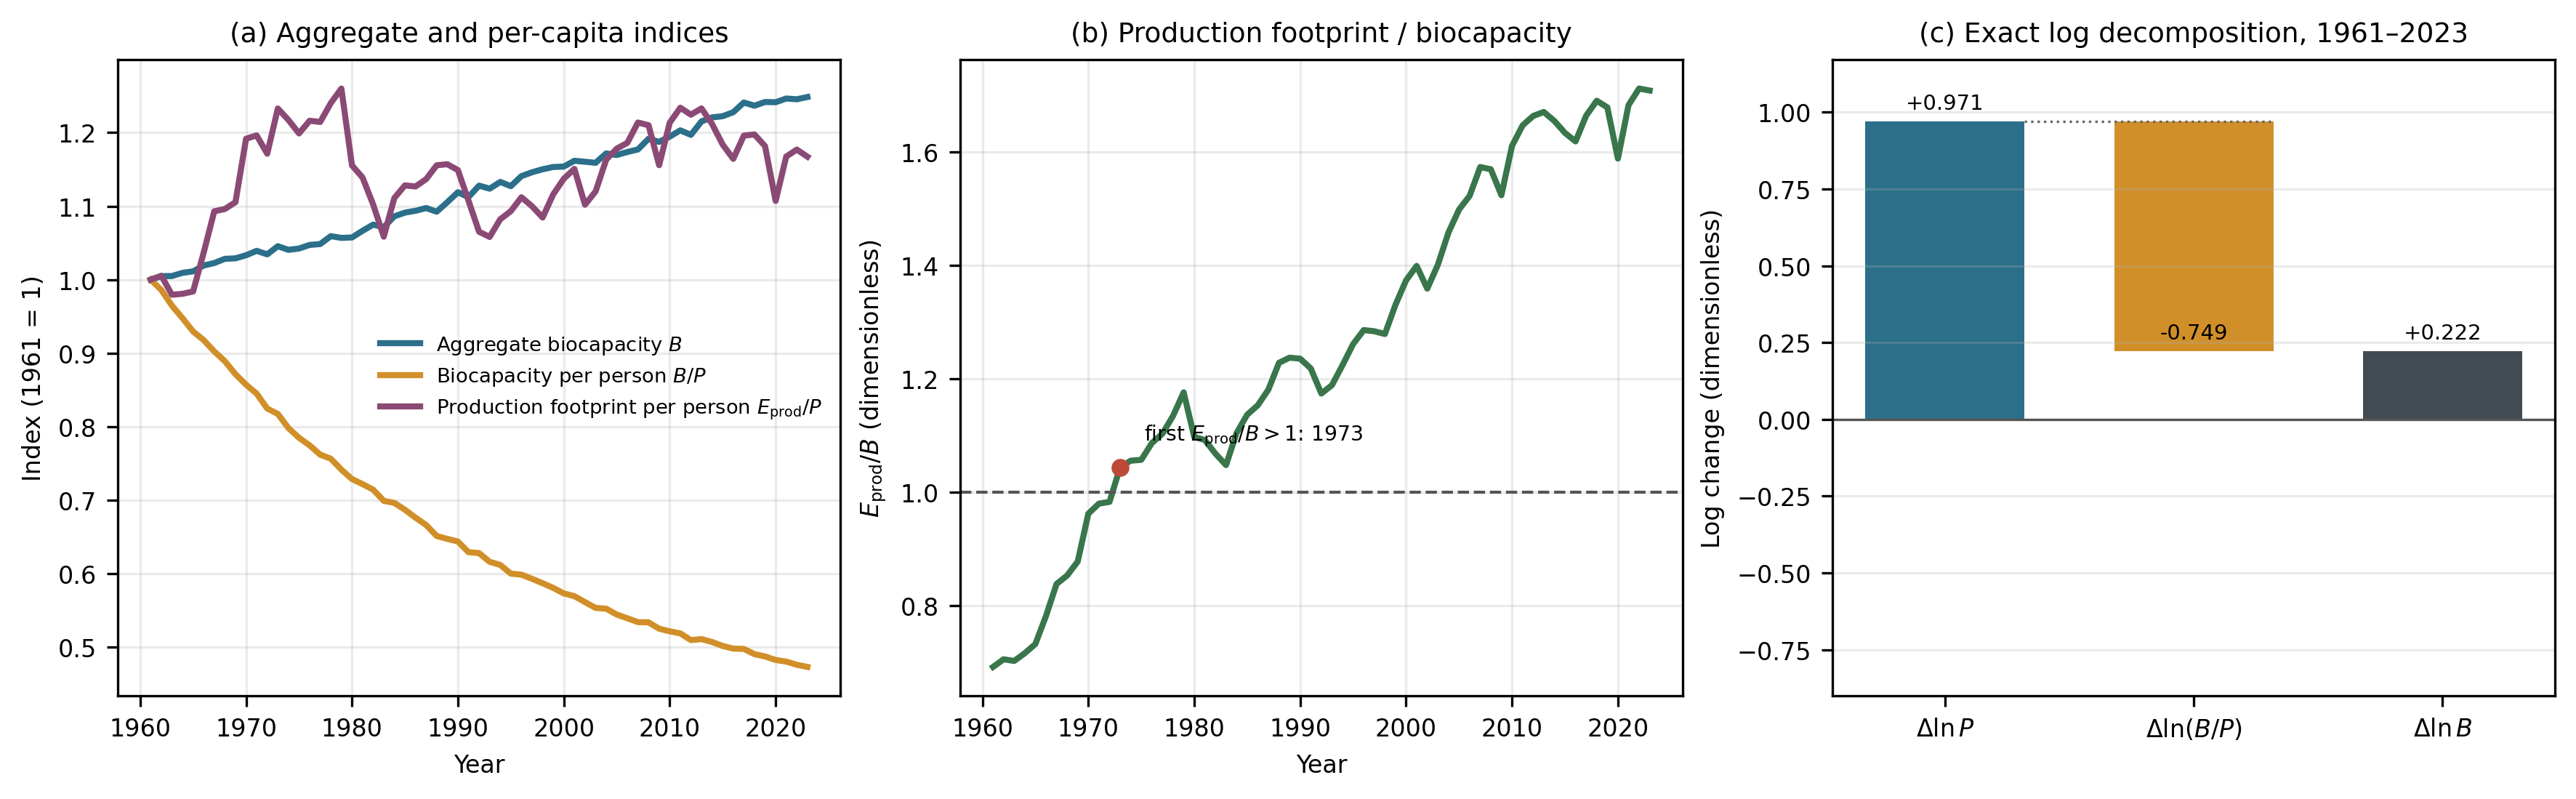
\includegraphics[width=\textwidth]{fig2_nfa_aggregation_face}
\caption{Aggregate and per-capita movements in NFA Edition 2026 (world, 1961--2023; complete observations). $B$ is total biocapacity, $E_{\mathrm{prod}}$ is the workbook's Global Ecological Footprint of Production, and $P$ is the single UN PopStat population series; per-capita values are calculated from totals. (a) Indices (1961 $=1$) of $B$, $B/P$, and $E_{\mathrm{prod}}/P$. (b) $E_{\mathrm{prod}}/B$, first above one in 1973. (c) Exact log identity $\Delta\ln B=\Delta\ln P+\Delta\ln(B/P)$. Account values are in gha; plotted indices, ratios, and log changes are dimensionless. The 2024--2025 estimated rows are excluded.}
\label{fig:aggregation}
\end{figure}

The land-type components make the NFA account composition explicit (Fig.~\ref{fig:composition}; Table~\ref{tab:nfa_components}). Cropland biocapacity contributes $+24.06$ percentage points to the $+24.86\%$ aggregate change, about $96.8\%$ of the net percentage change. Forest biocapacity contributes $-5.95$ points, grazing land $-0.27$, fishing grounds $-0.42$, and built-up land $+7.44$. The non-cropland account sum, which includes built-up land, is nearly flat ($1.0092\times$, or $+0.80$ points) only because it nets the built-up increase against declines in other categories. This is measured composition of NFA account values. It does not establish that forest biomass, soil condition, wetland extent, fish biomass, or the model's $A_c$ declined; built-up land is an accounting class, not ecological capital. Component values sum to total biocapacity within workbook rounding at both endpoints.

\begin{table}[!htbp]
\centering\footnotesize
\caption{NFA Edition 2026 biocapacity-account endpoint ratios and contributions. Contributions are $100\,[B_i(T)-B_i(1961)]/B(1961)$ percentage points; endpoint ratios are $B_i(T)/B_i(1961)$. The 2022 sensitivity is from the same edition. All entries are account values, not physical-stock measurements.}
\label{tab:nfa_components}
\begin{tabularx}{\textwidth}{@{}Xrrrr@{}}
\toprule
Component & \shortstack{2023\\ratio} & \shortstack{2023 contribution\\(pp of $B_{1961}$)} & \shortstack{2022 sensitivity\\ratio} & \shortstack{2022 contribution\\(pp of $B_{1961}$)} \\
\midrule
Cropland & 2.8701 & $+24.0577$ & 2.8514 & $+23.8183$ \\
Grazing land & 0.9828 & $-0.2688$ & 0.9815 & $-0.2890$ \\
Forest biocapacity & 0.8996 & $-5.9525$ & 0.9019 & $-5.8137$ \\
Fishing grounds & 0.9627 & $-0.4212$ & 0.9596 & $-0.4559$ \\
Built-up land$^{\dagger}$ & 8.7935 & $+7.4416$ & 8.6298 & $+7.2854$ \\
Non-cropland sum$^{\dagger}$ & 1.0092 & $+0.7990$ & 1.0083 & $+0.7267$ \\
\midrule
Total biocapacity & 1.2486 & $+24.8568$ & 1.2454 & $+24.5450$ \\
\bottomrule
\end{tabularx}
\begin{flushleft}\footnotesize
$^{\dagger}$Built-up land is not ecological capital; the non-cropland account sum includes it. Component sums match total biocapacity within workbook rounding. \end{flushleft}
\end{table}

\begin{figure}[!htbp]
\centering
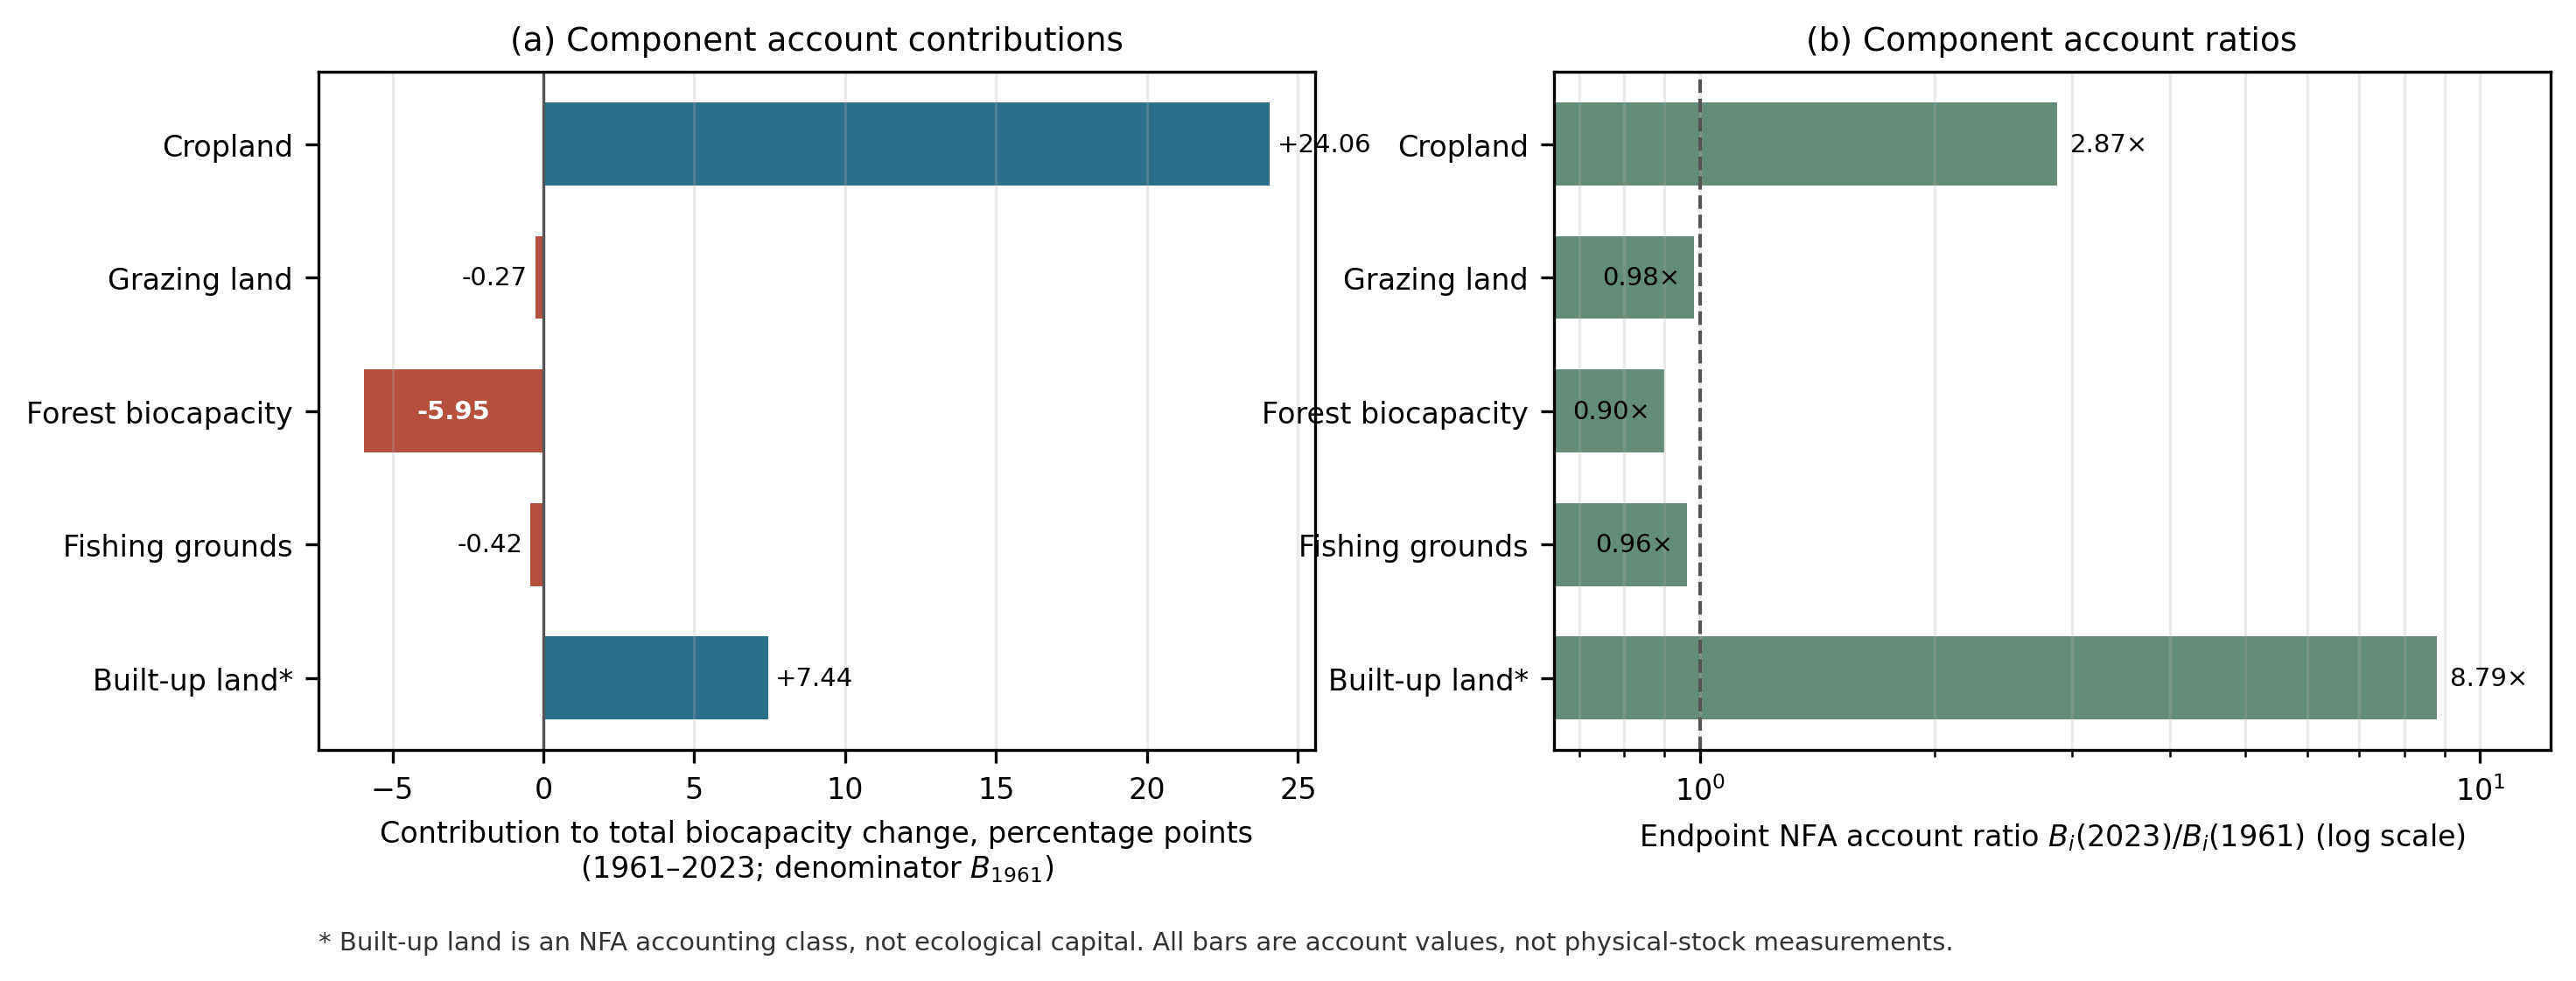
\includegraphics[width=0.95\textwidth]{fig3_composition_attribution}
\caption{NFA Edition 2026 land-type biocapacity-account changes, world, 1961--2023. (a) Component contributions in percentage points of $B_{1961}$. (b) Endpoint ratios $B_i(2023)/B_i(1961)$. “Forest biocapacity” is the workbook's exact label. All bars are account values, not measurements of physical stocks; built-up land is an NFA accounting class, not ecological capital.}
\label{fig:composition}
\end{figure}

A separate check uses external cropland area and cereal yield to construct a proxy for the fast-land contribution (SI~\S S5). With the 1961 NFA cropland share as the declared anchor, an exact log-change accounting split assigns $+0.268662$ to the cereal-yield index, $+0.037710$ to cropland area, and $-0.084375$ to the residual; the three terms sum to $\Delta\ln B=+0.221997$. This split is exact for the defined proxy, but it changes with the anchor and is not a physical-stock attribution.

\subsection{Falsifiable predictions}\label{sec:predictions}

The model yields the following testable predictions. Tests of land-class composition require observations of aggregate biocapacity, capital-land area, fast-land area, and relevant land-cover or yield proxies, rather than aggregate biocapacity alone.
\begin{enumerate}[label=P\arabic*.,leftmargin=2.2em]
\item \textbf{When the total can rise during conversion.} In the baseline frozen-demand run, a finite interval has $\dot A_c<0$ while $\dot B>0$ (Fig.~\ref{fig:model}a). The conversion contribution is positive exactly when $\dconv>0$, but other land flows, quality, debt, technology, and restoration determine the net change in $B$. With baseline availability shares $\sigma_f=\sigma_c=1$, conversion requires demand to exceed total biocapacity, or $R_B=E/B>1$. With reserved shares below one, the extension can permit conversion even when $R_B\le1$; this is not a baseline result. The composition mask is the pattern $B$ rising while $A_c$ falls; the distinct liquidation mask is $E$ steady while $A_c$ falls. The patterns can overlap, and neither label is a synonym for the other. The sign of $\dconv$ describes the conversion contribution, not necessarily the net change in $B$ when other terms are active.
\item \textbf{How long the pattern lasts.} Its duration depends on the slow return rate $\lambda_1$ (and on $\tconv$, $\mu$, $\eta_f$, and $b_c/b_f$); its size depends on $\dconv$ and the initial shortfall. It is not set by a universal time horizon. In the baseline run, most conversion occurs within one to two e-folding times—the time for the remaining gap to shrink by a factor of $e$.
\item \textbf{No fold-type early warning in the reduced model.} The return time does not grow as demand approaches the ceiling, and the depth of drawdown changes continuously with demand (Fig.~\ref{fig:model}c). Instead, the modeled signal is $A_c$ approaching its minimum. The model does not predict a fold-related warning before this boundary is reached.
\item \textbf{A population threshold with weak delay sensitivity in the tested range.} The initial population at which a run approaches the capital-land minimum rises with starting capital-land area (Table~\ref{tab:model}b). At $A_{c0}=1.0$\,ha, the $10^{-6}$\,ha proximity value changes by at most $0.001$\,cap across $\tau_g=5$, $20$, and $40$\,yr (SI Table S2). This finite-range comparison does not establish delay invariance; the small change is consistent with the modest regenerative contribution and monotone quality trajectory in the baseline.
\item \textbf{Recovery needs a return flow.} Reducing demand alone does not restore capital-land area. An explicit restoration flow is required; a surplus-gated flow is inactive during shortfall, while a deficit-gated flow can deepen the provision deficit.
\end{enumerate}
The predictions cannot be tested from aggregate $B$ alone. Tests of the composition mechanism require independent observations or defensible proxies for $A_c$ and fast-land yield $b_f$; tests of the delay, recovery, and demand-threshold predictions require corresponding trajectories and intervention or demographic data.
